

\documentclass[11pt, oneside]{article}   	% use "amsart" instead of "article" for AMSLaTeX format
\usepackage{geometry}                		% See geometry.pdf to learn the layout options. There are lots.
\geometry{letterpaper}                   		% ... or a4paper or a5paper or ... 
%\geometry{landscape}                		% Activate for for rotated page geometry
%\usepackage[parfill]{parskip}    		% Activate to begin paragraphs with an empty line rather than an indent
\usepackage{graphicx}				% Use pdf, png, jpg, or eps with pdflatex; use eps in DVI mode
\usepackage{listings}			         % For showing code			
								% TeX will automatically convert eps --> pdf in pdflatex		
\usepackage{amssymb}

\title{Example Guide for MEDYAN \textbf{v4.0}}
\author{Papoian Lab, University of Maryland}
\date{}							% Activate to display a given date or no date

\begin{document}
\maketitle
%\section{}
%\subsection{}

\tableofcontents
\newpage

\section{Introduction}

Examples can be found in \texttt{InstallDirectory/examples}, and will grow with the increasing application of MEDYAN to various scientific projects. Each example includes a \texttt{SystemFile} as well as chemical input file. To run a given example once the MEDYAN executable is created, go to \texttt{InstallDirectory/src} and run the following:\newline

\indent \texttt{> ./MEDYAN -s InstallDirectory/examples/<ExampleFolder>/SystemFile}\newline
\indent\indent \texttt{-i InstallDirectory/examples/<ExampleFolder>/  -o <OutputDirectory>}\newline

\noindent where \texttt{<ExampleFolder>} is the specific example folder desired, and \texttt{<OutputDirectory>} is the directory of the desired output. See the usage guide for more details on these files and directories.

\section{Example 1: A simple actomyosin network}

This example is aimed at setting up disordered actomyosin networks similar to our recently published paper [1]. This system contains actin filaments with their constituent monomers, as well as $\alpha$-actinin cross-linking protein and non-muscle myosin IIA (NMIIA) motors in a 1 $um^3$ cubic boundary. The example files can be found at \texttt{InstallDirectory/examples/ex1}.

\subsection{Input file parameters}

\subsubsection{systeminput.txt}

This file contains key parameters defining the system configuration, sectioned by comments. For a full list of these parameters, see the usage guide at \texttt{InstallDirectory/docs/UsageGuide.pdf}.

\begin{itemize}
\item \texttt{\textbf{GEOMETRY}} - This section specifies parameters of the reaction-diffusion compartment grid, including the compartment size and the number of compartments in each dimension (\texttt{COMPARTMENTSIZE} and \texttt{N}) to be 500 $nm$ in length in all directions in a 2x2x2 compartment grid. Currently, the number of dimensions must be 3. Cylinder and monomer sizes are also defined, which controls the level of polymer coarse-graining. It is set to 27 and 2.7 $nm$, respectively. The boundary shape chosen is cubic, which simply covers the planes defined by the compartment grid.

\item \texttt{\textbf{MECHANICS}} - Here, all mechanical force field types and parameters for actin filaments, $\alpha$-actinin, and NMIIA are defined. For a choice of these parameters, which mimics the mechanical properties of the actomyosin elements, see [1]. The algorithm section specifies the type of conjugate gradient used (currently \texttt{POLAKRIBIERE}) as well as mechanical minimization parameters that we have chosen. We suggest not changing these as they have given optimal efficiency and accuracy for this system configuration.

\item \texttt{\textbf{CHEMISTRY}} - Although there is a separate chemistry input file which is defined in this section, the chemistry section in this file defines the algorithm parameters for stochastic reaction-diffusion simulation, including run and snapshot times, as well as other update frequencies, including mechanical minimization and neighbor list updates. This section also lists the number of each chemical species which should match the chemistry input file \texttt{chemistryinput.txt}. This system is set to run for 2000 $s$, taking 10 $s$ snapshots and performing mechanical equilibration and neighbor list updating every 0.05 $s$.

\item \texttt{\textbf{DYNAMIC RATE CHANGING}} - This section defines mechanochemical feedback relationships between simulation elements, including polymers, cross-linkers, and motors. For actin filaments in this case, a brownian ratchet polymerization model is used with characteristic distance 2.7 $nm$. For $\alpha$-actinin, a slip bond was used with characteristic unbinding distance 0.24 $nm$. For NMIIA, a more complicated catch bond was implemented for low-duty motor ensembles. For details on any of these mechanochemical relationships, see [1].

\item \texttt{\textbf{INITIALIZATION}} - Initial filaments in the system, which will be arranged randomly throughout the volume. Currently, 50 filaments will be created, all with an initial size of 1 cylinder (27 $nm$).

\end{itemize}

\subsubsection{chemistryinput.txt}

This file contains key parameters defining the system's specific chemical configuration. For a full list of these parameters, see the usage guide at \texttt{InstallDirectory/docs/UsageGuide.pdf}. This file must be listed in the system configuration file to be parsed.

\begin{itemize}

\item \texttt{\textbf{SPECIES}} - All chemical species, regardless of type, are initialized in this file. This system contains diffusing actin = 20 $\mu M$ (\texttt{AD}) as well as diffusing $\alpha$-actinin ($R_{\alpha:a}=0.1$) and NMIIA  ($R_{m:a}=0.02$) (\texttt{LD} and \texttt{MD}) with specified copy number in the simulation volume, as well as diffusion rates and release times as defined in the usage guide. Copy numbers can be converted to molar concentrations using the known system volume. The qualifier \texttt{REG} tells the program to not use any special counting of these species that may optimize the reaction-diffusion simulation. Besides diffusing species, filament species for each filament desired must be defined, as well as plus and minus end species. These species names are eventually used in the reaction section below. Lastly, for binding molecules, a binding site must be specified which is an empty bound site for that species on a given filament.

\item \texttt{\textbf{REACTIONS}} - All chemical reactions in the system including the (de)polymerization of actin filaments at both ends, as well as $\alpha$-actinin and NMIIA binding, as well as NMIIA walking, are listed here as defined in the usage guide. Each reaction has its own kinetic rate constant and characteristic distances; for example, $\alpha$-actinin binding occurs at 0.009 $s^{-1}$ between distances of 30 and 40 $nm$. Binding reactions, including $\alpha$-actinin and NMIIA, have both a binding and unbinding rate defined, as well as binding ranges.

\end{itemize}

\subsection{Running simulation}

Run the following command to run the example simulation after compiling MEDYAN in \texttt{InstallDirectory/src}:\\

\indent \texttt{> ./MEDYAN -s InstallDirectory/examples/ex1/systeminput.txt}\newline
\indent\indent \texttt{-i InstallDirectory/examples/ex1/  -o InstallDirectory/examples/ex1/}\newline

\noindent This will place output files in the same folder as the input. Expect the simulation to take up to 12 hours (on a typical ~2.8GHz processor), so detaching the process from an active terminal window is highly recommended.

\subsection{Visualization and analysis}

This section will assume that the user has MayaVi and interactive Python set up correctly; see \texttt{InstallDirectory/docs/UsageGuide.pdf} for a list of requirements and installation dependencies for these packages. 

\subsubsection{Running visualizer}

To run the visualizer \texttt{AnimateTrajectory.py} on the output, which will produce animations of each trajectory snapshot:

\begin{itemize}
\item Set the trajectory file's path in line 7 of the script.
\item Set the grid size minimum and maximum to be 1000 $nm$ and 0 $nm$; this is the size of the simulated domain.
\item Define any colors and labels desired in lines 314-357 of the script.
\end{itemize}

This output can then be shown by using the \texttt{show\_snapshot()} and \texttt{anim()} functions after running \texttt{run -i AnimateTrajectory.py} in an interactive Python session, which are discussed in \texttt{InstallDirectory/docs/UsageGuide.pdf}. Sample output is shown below. 

\begin{figure}[h]
\caption{A sample trajectory snapshot visualized with \texttt{AnimateTrajectory.py}}
\centering
%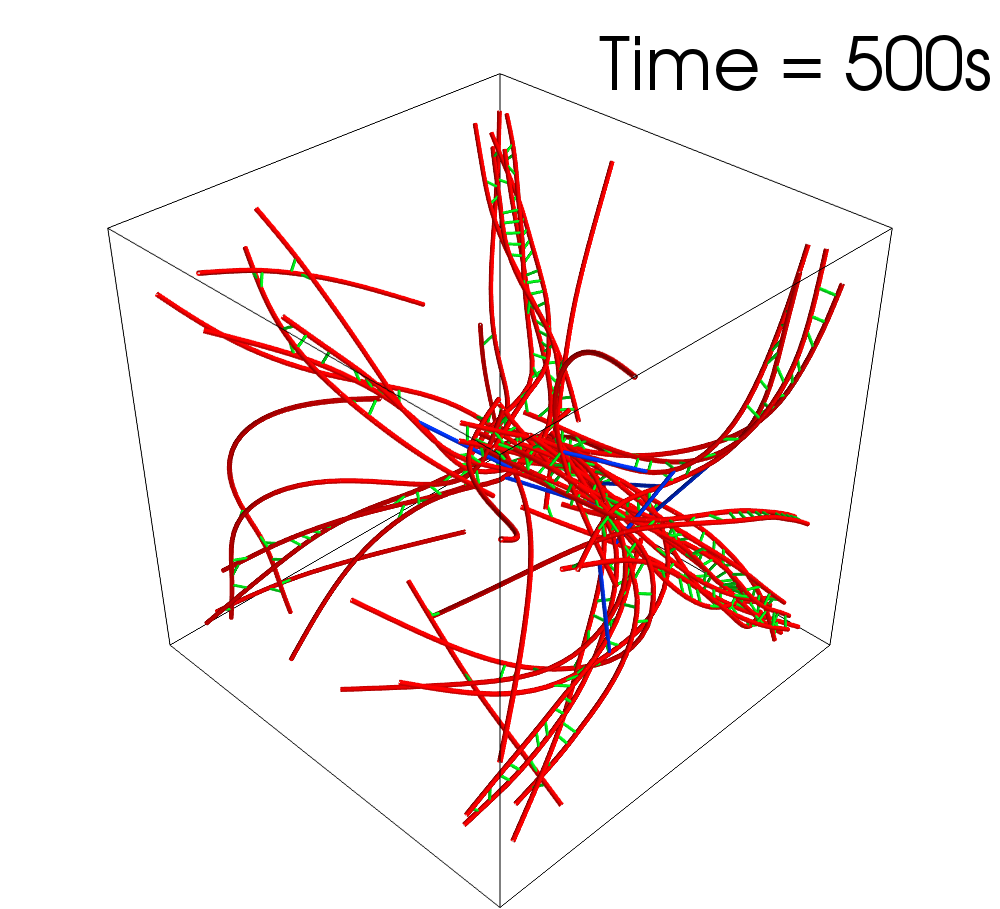
\includegraphics[width=0.8\textwidth]{SampleTraj}
\end{figure}

\subsubsection{Simple analysis: $R_g$ and $S$}

To run our interactive analysis script \texttt{ex1analysis.py} on the output, producing plots for the network's radius of gyration $R_g$ and orientational order parameter $S$ over time, which are defined in [1]:\\

\indent \texttt{> run -i ex1analysis.py}\\
\indent \texttt{> snapshotlist = readTrajectory('InstallDirectory/examples/ex1/snapshot.traj')}\\
\indent \texttt{> plotRg(snapshotlist)}\\
\indent \texttt{> plotOrderParameter(snapshotlist)}\\

\subsection{Other exercises}

We leave it as an exercise to the user, after completing the above simulation and brief analysis and visualization, to reproduce the actomyosin transition to contraction above a threshold $\alpha$-actinin concentration (Figure 10 in [1]) by varying the initial copy number of $\alpha$-actinin relative to a fixed actin concentration (currently $R_{\alpha:a}=0.1$) and keeping all other parameter values fixed. This should produce $R_g$ values that monotonically increase with $\alpha$-actinin concentration as in [1], with a sharp increase in contraction above $R_{\alpha:a}=0.05$.

To see this dependence, multiple trajectories may be required for each $\alpha$-actinin concentration. This can be read, after generating multiple trajectories, with the following functions, which are similar to the ones presented above but read and average over all trajectory time points:\\

\indent \texttt{> run -i ex1analysis.py}\\
\indent \texttt{> snapshotlists = readTrajectories(fileDirectory = 'InstallDirectory/examples/ex1/')}\\
\indent \texttt{> plotRgs(snapshotlists)}\\
\indent \texttt{> plotOrderParameters(snapshotlists)}\\

\noindent Calling all plotting functions multiple times will overlay the newly generated plot onto an already existing one, allowing the plotting of multiple concentration configurations in a single figure. Below is the result from [1] for reference.

\begin{figure}[h]
\caption{Figure 8 from [1], showing transition to contractile structures above $R_{\alpha:a}=0.05$.}
\centering
%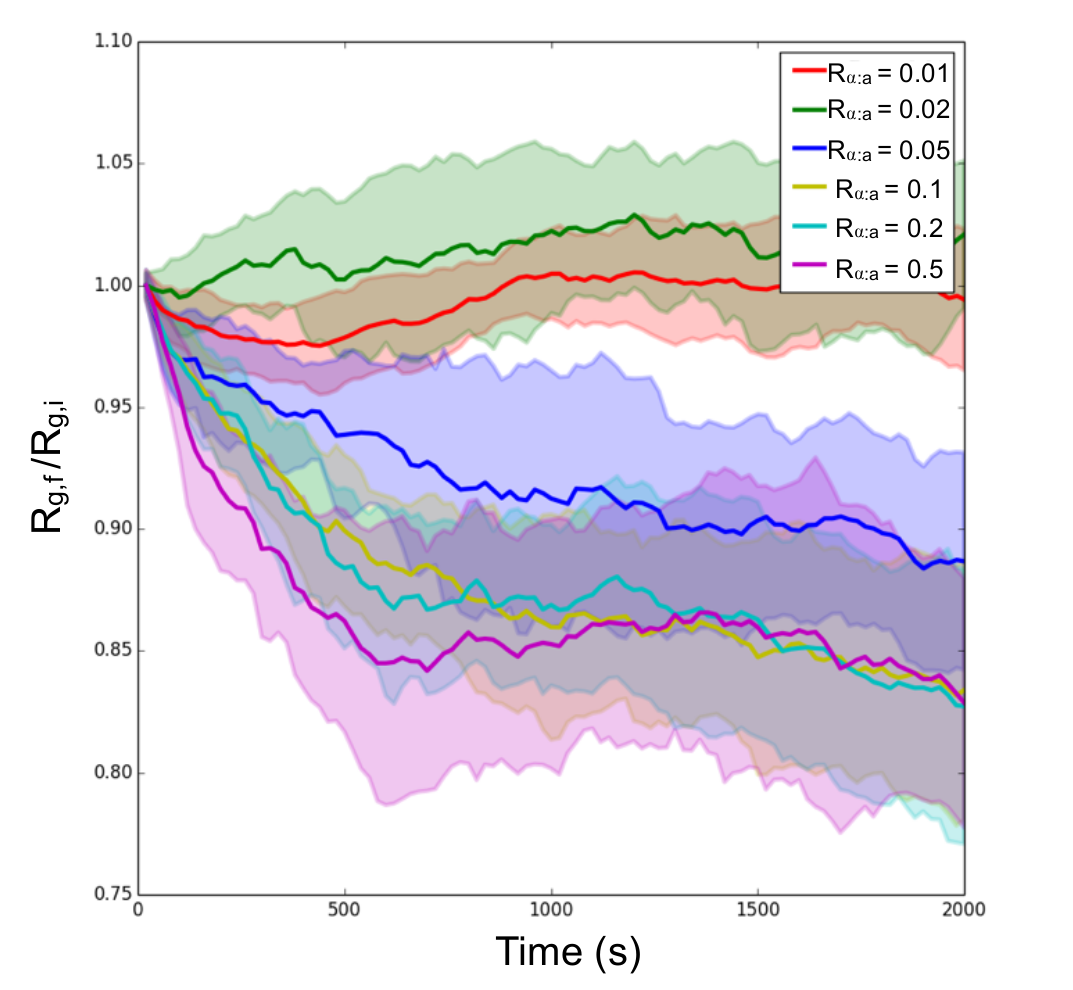
\includegraphics[width=0.8\textwidth]{Fig8}
\end{figure}

\section{References}

[1] Popov K, Komianos J, and GA Papoian. ``MEDYAN: Mechanochemical Simulations 
\indent of Contraction and Polarity Alignment in Actomyosin Networks." PLoS Computational \indent Biology 2016; 12(4): e1004877. doi:10.1371/journal.pcbi.1004877

\end{document}